\chapter{Introduction}
\section{Présentation du projet}
\paragraph{Objectif}
Mettre en place, évaluer et comparer différents outils permettant de gérer de manière
centralisée et automatisée une infrastructure basée sur des machines virtuelles: Ganeti,
OpenXenManager, virt-manager, Archipel...
\section{Introduction à la virtualisation}

\chapter{Ganeti}
\section{Introduction}
Ganeti est un outil de gestion de machines virtuelles se basant sur les technologies de virtualisation existantes comme XEN et KVM.\\
Ganeti nécessite un logiciel de virtualisation pré-installé sur les serveurs afin de pouvoir fonctionner. Une fois installé, 
l'outil prendra en charge la partie gestion des instances virtuelles (Xen DomU), par exemple, la gestion de création de disque, 
l'installation du système d'exploitation (en coopération avec les scripts d'installation du système d'exploitation 
spécifique), et le démarrage, l'arrêt, le basculement entre les systèmes physiques. Il a été conçu pour faciliter la gestion de 
cluster de serveurs virtuels et de fournir une récupération rapide et simple.
\section{Installation}
\section{Utilisation}


\section{Présentation de Grid5000}
Aujourd’hui, grâce à Internet, il est possible
d’interconnecter des machines du monde entier pour
traiter et stocker des masses de données. Cette collection
hétérogène et distribuée de ressources de stockage et de
calcul a donné naissance à un nouveau concept : les
grilles informatiques. L’idée de mutualiser les ressources
informatiques vient de plusieurs facteurs, évolution de la
recherche en parallélisme qui, après avoir étudié les
machines homogènes, s’est attaquée aux environnements
hétérogènes puis distribués ; besoins croissants des
applications qui nécessitent l’utilisation toujours plus
importante de moyens informatiques forcément répartis.
La notion de grille peut avoir plusieurs sens suivant le
contexte : grappes de grappes, environnements de type
GridRPC (appel de procédure à distance sur une grille).,
réseaux pair-à-pair, systèmes de calcul sur Internet, etc...
Il s’agit d’une manière générale de systèmes dynamiques,
hétérogènes et distribués à large échelle. Un grand
nombre de problématiques de recherche sont soulevées
par les grilles informatiques. Elles touchent plusieurs
domaines
de l’informatique :algorithmique,
programmation, intergiciels, applications, réseaux.
L’objectif de GRID’5000 est de construire un instrument
pour réaliser des expériences en informatique dans le
domaine des systèmes distribués à grande échelle (GRID).
Cette plate-forme, ouverte depuis 2006 aux chercheurs de
la communauté grille, regroupe un certain nombre de sites
répartis sur le territoire national. Chaque site héberge une
ou plusieurs grappes de processeurs. Ces grappes sont
alors interconnectées via une infrastructure réseau dédiée
à 10 Gb/s fournie par RENATER. À ce jour, GRID’5000
est composé de 9 sites: Lille, Rennes, Orsay, Nancy,
Bordeaux, Lyon, Grenoble, Toulouse et Nice. Début 2007,
GRID’5000 regroupait plus de 2500 processeurs et près
de 3500 cœurs.

\newpage
\begin{center}
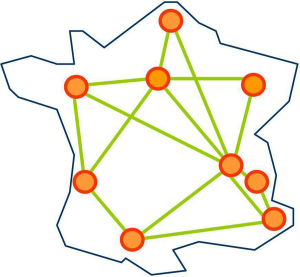
\includegraphics{images/g5k.png}
\underline{\textit{Architecture Grid5000}}
\end{center}
